\documentclass{kththesis}

\usepackage{csquotes} % Recommended by biblatex
\usepackage{biblatex}
\addbibresource{references.bib} % The file containing our references, in BibTeX format

\usepackage{mathtools, graphicx, hyperref, amssymb, algorithm2e}
\usepackage[utf8]{inputenc}
\usepackage[T1]{fontenc}
\usepackage{listings}
\usepackage{bcprules}
\usepackage{multicol}
\usepackage{tikz}
\usepackage{mathrsfs}

\usepackage{inconsolata}

% Configuration of font and stuff for listings
\usepackage{color}
\newcommand{\codestyle}{\small\ttfamily}
\newcommand{\nstyle}{\small\ttfamily\color{grey}}
\definecolor{grey}{rgb}{0.5,0.5,0.5}
\lstset{
%  frame=tb,
  language=scala,
%  aboveskip=3mm,
%  belowskip=3mm,
%  lineskip=-0.1em,
  showstringspaces=false,
  columns=[c]fixed,
  basewidth={0.5em,0.4em},
  mathescape=true,
  numbers=left,
  numberstyle=\nstyle,
  basicstyle=\codestyle
}  

% Other listings-related settings from
% http://lampsvn.epfl.ch/trac/scala/export/26099/scala-tool-support/trunk/src/latex/scaladoc.sty
% activate the language and predefine settings
%\lstset{
%    language=Scala,%
%    xleftmargin=4mm,%
%    aboveskip=3mm,%
%    belowskip=3mm,%
%    fontadjust=true,%
%    columns=[c]fixed,%
%    keepspaces=true,%
%    basewidth={0.58em, 0.53em},%
%    tabsize=2,%
%    basicstyle=\renewcommand{\baselinestretch}{0.95}\ttfamily,%
%    commentstyle=\itshape,%
%    keywordstyle=\bfseries,%
%    mathescape=true,%
%    escapechar=¤,%
%    captionpos=b,%
%    framerule=0.3pt,%
%    firstnumber=0,%
%    numbersep=1.5mm,%
%    numberstyle=\tiny,%
%}
%
%\lstdefinestyle{floating}{%
%    xleftmargin=10pt,%
%    xrightmargin=5pt,%
%    aboveskip=4mm,%
%    belowskip=4mm,%
%    fontadjust=true,%
%    columns=[c]flexible,%
%    keepspaces=true,%
%    basewidth={0.5em, 0.425em},%
%    tabsize=2,%
%    basicstyle=\renewcommand{\baselinestretch}{0.95}\ttfamily,%
%    commentstyle=\rm,%
%    keywordstyle=\bfseries,%
%    mathescape=true,%
%    captionpos=b,%
%    framerule=0.3pt,%
%    firstnumber=0,%
%    numbersep=1.5mm,%
%    numberstyle=\tiny,%
%    float=tbp,%
%    frame=tblr,%
%    framesep=5pt,%
%    framexleftmargin=3pt,%
%    abovecaptionskip=\smallskipamount,%
%    belowcaptionskip=\smallskipamount,%
%} % to define: caption, label


% Definitions of commands
%% This file is for definitions of commands

\newcommand{\image}{\text{Im }}
\newcommand{\reals}{\mathbb{R}}
\newcommand{\integers}{\mathbb{Z}}
\newcommand{\ratio}{\mathbb{Q}}
\newcommand{\ilc}[1]{\lstinline[keepspaces=true]$#1$}
\newcommand{\ilclang}[2]{\lstinline[keepspaces=true,language=#1]$#2$}
\newcommand{\lacasa}{\textsc{LaCasa}}
\newcommand{\CLCone}{\textsc{CLC}$^1$}
\newcommand{\scrule}[3]{\infrule[\textsc{#1}]{#2}{#3}}
\newcommand{\scax}[2]{\infax[\textsc{#1}]{#2}}
\newcommand{\stof}{<:}
\newcommand{\lub}{\sqcup}

\newcommand{\LatType}{\mbox{$\mathcal{L}$}}
\newcommand{\AnyRefType}{\mbox{$\mathsf{AnyRef}$}}
\newcommand{\CellType}{\mbox{$\mathsf{Cell}$}}
\newcommand{\NullType}{\mbox{$\mathsf{Null}$}}

\newcommand{\LatVals}{\mbox{$\mathscr{L}$}}

% Commands for writing language syntax

\newcommand{\ClassDef}[4]{\mbox{\texttt{class}~$#1$~\texttt{extends}~$#2$~\texttt{\{}$#3$~$#4$\texttt{\}}}}
\newcommand{\VarDecl}[2]{\mbox{\texttt{var}~$#1$~\texttt{:}~$#2$}}
\newcommand{\MethodDef}[5]{\mbox{\texttt{def}~$#1$\texttt{(}$#2$~\texttt{:}~$#3$\texttt{)}~\texttt{:}~$#4$~\texttt{=}~$#5$}}
\newcommand{\Let}[3]{\mbox{\texttt{let}~$#1$~\texttt{=}~$#2$~\texttt{in}~$#3$}}
\newcommand{\NullVal}{\mbox{\texttt{null}}}
\newcommand{\FSel}[2]{\mbox{$#1$\texttt{.}$#2$}}
\newcommand{\FAss}[3]{\mbox{$#1$\texttt{.}$#2$~\texttt{=}~$#3$}}
\newcommand{\New}[1]{\mbox{\texttt{new}~$#1$}}
\newcommand{\NewCell}{\mbox{\texttt{new}~\texttt{Cell}}}
\newcommand{\Call}[3]{\mbox{$#1$\texttt{.}$#2$\texttt{(}$#3$\texttt{)}}}
\newcommand{\Put}[2]{\mbox{$#1$~\texttt{put}~$#2$}}
\newcommand{\When}[3]{\mbox{\texttt{when}~$#1$~\texttt{pass}~$#2$~\texttt{then}~$#3$}}
\newcommand{\Capt}[2]{\mbox{$#1$~\texttt{=}~$#2$}}
\newcommand{\CB}[3]{\mbox{($#1$, $#2$~$\Rightarrow$~$#3$)}}
\newcommand{\This}{\mbox{\texttt{this}}}


% Typing relation
\newcommand{\TypeRel}[4]{\mbox{$#1;#2\vdash#3:#4$}}

\newcommand{\RuleSpace}{\vspace{0.8em}}


\newcommand{\nocap}{\mbox{$\epsilon$}}
\newcommand{\ocap}{\mbox{$ocap$}}

\newcommand{\LaCasa}{\mbox{LaCasa}}
\newcommand{\RACL}{\mbox{RACL}}

% Reduction relations
\newcommand{\FRedTo}{\mbox{$\rightarrow$}}
\newcommand{\FSRedTo}{\mbox{~$\twoheadrightarrow$~}}
\newcommand{\ProcsRedTo}{\mbox{~$\Rrightarrow$~}}

\newcommand{\Frame}[3]{\mbox{$\langle #1, #2 \rangle^{#3}$}}
\newcommand{\sFrame}[2]{\Frame{#1}{#2}{s}}
\newcommand{\sframe}[1]{\mbox{$\langle #1 \rangle^s$}}
\newcommand{\xframe}[1]{\mbox{$\langle #1 \rangle$}}

%\newcommand{\Obj}[2]{\mbox{$\langle #1, #2 \rangle$}}
\newcommand{\Obj}[1]{\mbox{$\langle #1 \rangle$}}
\newcommand{\Cell}[1]{\mbox{$\langle \CellType{}, #1 \rangle$}}
\newcommand{\Error}{\mbox{{\bf error}}}

\newcommand{\typeOf}{\mbox{$\mathrm{typeOf}$}}
\newcommand{\dom}{\mbox{$\mathrm{dom}$}}
\newcommand{\fields}{\mbox{$\mathrm{fields}$}}
\newcommand{\ftype}{\mbox{$\mathrm{ftype}$}}
\newcommand{\ErrType}{\mbox{$T_{\text{err}}$}}

\newcommand{\isolated}{\mbox{$\mathrm{isolated}$}}
\newcommand{\accRoot}{\mbox{$\mathrm{accRoot}$}}
\newcommand{\accRoots}{\mbox{$\mathrm{accRoots}$}}
\newcommand{\csep}{\mbox{$\mathrm{csep}$}}
\newcommand{\isolation}{\mbox{$\mathrm{isolation}$}}
\newcommand{\reach}{\mbox{$\mathrm{reach}$}}
\newcommand{\ocrloc}{\mbox{$\mathrm{ocr}$}}
\newcommand{\ocr}{\mbox{\bf ocr}}
\newcommand{\gsep}{\mbox{\bf gsep}}
\newcommand{\stateok}{\mbox{\bf ok}}
\newcommand{\tsep}{\:\:}
\newcommand{\reachable}{\mbox{$\mathrm{reachable}$}}

\newcommand{\noSpawn}{\mbox{$\mathrm{noSpawn}$}}


\newcommand{\Graph}{\ensuremath{\mathscr{G}}}
\newcommand{\FieldNames}{\ensuremath{\mathscr{F}}}
\newcommand{\Values}{\ensuremath{\mathscr{V}}}


\title{This is the English title}
\alttitle{Detta är den svenska översättningen av titeln}
\author{Ellen Arvidsson}
\email{magarv@kth.se}
\supervisor{Philipp Haller}
\examiner{Mads Dam}
\programme{Master in Computer Science}
\school{School of Electrical Engineering and Computer Science}
\date{\today}


\begin{document}

% Frontmatter includes the titlepage, abstracts and table-of-contents
\frontmatter

\titlepage

\begin{abstract}
  English abstract goes here.

\end{abstract}


\begin{otherlanguage}{swedish}
  \begin{abstract}
    Träutensilierna i ett tryckeri äro ingalunda en oviktig faktor,
    för trevnadens, ordningens och ekonomiens upprätthållande, och
    dock är det icke sällan som sorgliga erfarenheter göras på grund
    af det oförstånd med hvilket kaster, formbräden och regaler
    tillverkas och försäljas Kaster som äro dåligt hopkomna och af
    otillräckligt.
  \end{abstract}
\end{otherlanguage}


\tableofcontents


% Mainmatter is where the actual contents of the thesis goes
\mainmatter

\chapter{Introduction}
\label{cha:introduction}

%We use the \emph{biblatex} package to handle our references.  We therefore use the
%command \texttt{parencite} to get a reference in parenthesis, like this
%\parencite{heisenberg2015}.  It is also possible to include the author
%as part of the sentence using \texttt{textcite}, like talking about
%the work of \textcite{einstein2016}.

\chapter{Background}
\label{cha:background}

\section{Language Syntax}
\label{sec:language_syntax}

% Describe the foundations of syntaxes for languages: BNF, ANF

\section{Language Semantics}
\label{sec:language_semantics}

% Describe small step operational semantics

\section{Type Systems}
\label{sec:type_systems}

% Describe basic type systems and properties that should hold e.g. 
% TODO Preservation and Progress


\chapter{Related Work}
\label{cha:related_work}

\section{LVars}
\label{sec:lvars}

% Should describe the basic ideas of LVars and also mention that there are
% problems with the proof and hint of bigger problems.

\section{Reactive Async}
\label{sec:reactive_async}

% Should describe reactive async. There are multiple issues with this system,
% e.g. that great care has to be taken in order to make the system
% deterministic, e.g. make sure that only certain types of operations are
% allowed in the callbacks.

\section{LaCasa}
\label{sec:lacasa}

% Describes the basic ideas of lacasa and the idea of using OCAP constraints to % assure determinism

\section{Spores}
\label{sec:spores}

% Describe the basic ideas of spores: (dis)allow certain types of captures to
% enforce certain properties



\chapter{Challenges of Deterministic Concurrency}
\label{cha:challenges}

% Describe the problem of arbitrary reading data from an object that is
% concurrently being changed. Describe the idea of threshold reads and how it
% can be utilized to get determinism.

\chapter{Core Language}%
\label{cha:core_language}

In this chapter a basic core language is introduced. It will build a lot upon
the core language of LaCasa and incorporate features of LVish. In the end we will
have an object oriented language incorporating many of the features of LVish with
a type system enforcing OCAP properties, much like the system of LaCasa.

\section{Syntax}
\label{sec:syntax}

The language which we shall call Reactive Async Core Language (RACL) has a big
similarity with the core language from LaCasa. Many expressions are the same
except for a few removals and additions. The language grammar is defined in
Figure~\ref{fig:racl_grammar}. It is a simple object oriented language which is
parameterized on the lattice \LatVals{}.

\begin{figure}
  \centering
  $\begin{array}{lll@{\hspace{4mm}}l}
    p &::= &\overline{cd}~\overline{vd}~t  & \mbox{Program} \\
    cd &::= &\texttt{class}~C~\texttt{extends}~D~\{\overline{fd}~\overline{md}\}
    & \mbox{Class} \\
    vd,fd &::= &\texttt{var}~f~:~\tau & \mbox{Variable/Field} \\
    md &::= &\texttt{def}~m(x: \sigma):~\tau = t & \mbox{Method}\\
    &&&\\
    \sigma,\tau & ::= & & \mbox{Types} \\
    & & C, D & \mbox{Class types} \\ 
    &| & \CellType & \mbox{Cell type} \\
    %&| & \NullType & \mbox{Null type} \\
    &| & \LatType & \mbox{Lattice value type} \\
    &&&\\
    t &::=& & \mbox{Terms} \\
    & & x & \mbox{Variable} \\
    &|& \texttt{let}~x = e~\texttt{in}~t &\mbox{Let binding} \\
    &&&\\
    e &::=& & \mbox{Expression} \\
    & & l & \mbox{Lattice value} \\
    &|& \texttt{null} & \mbox{Null reference} \\
    &|& x &\mbox{Variable} \\
    &|& x.f &\mbox{Field selection} \\
    &|& x.f = y & \mbox{Field assignment} \\
    &|& \texttt{new}~C & \mbox{Class instance creation} \\
    &|& \texttt{new}~\texttt{Cell} & \mbox{Cell instance creation} \\
    &|& x.m(y) & \mbox{Method invocation} \\
    &|& x~\texttt{put}~y & \mbox{Cell value update} \\
    &|& \texttt{when}~x~\texttt{pass}~y~\texttt{then}~(\overline{cap}, z
    \Rightarrow t) & \mbox{Dependency creation} \\
    &&&\\
    cap & ::= & x = y & \mbox{Variable capture} \\
  \end{array}$
  \caption{Grammar of RACL}
  \label{fig:racl_grammar}
\end{figure}

We can see that a program $p$ consists of a sequence of class definitions
$\overline{cd}$, a sequence of variable declarations $\overline{vd}$ and a term
$t$. A class definition $cd$ consists of a name specifier $C$, inheritance
specifier $D$, field declarations $\overline{fd}$ and method definitions
$\overline{md}$. Variable and field declarations both have the same form
consisting of a name specifier $f$ and a type $\tau$. Method definitions are
also standard, with one thing to note that all methods takes exactly one input.
More complicated inputs can be constructed using a container class.

The type specifiers $\sigma$ and $\tau$ can take on the values as specified.
Note that we have the special \CellType{} and \LatType{} types which are meant
to represent the cells of reactive async and values from the used lattice. Types
will be discussed more in Section~\ref{sec:type_system}.

As with LaCasa, the terms of RACL are written in A-normal form (i.e.\ every
subexpression is named). Most of the expressions should be self-explanatory.
However, note for example that we have a separate instance creation expression
for cells, an expression for updating the value of a cell aswell as an
expression for creating dependencies between cells. The dependency creation
expression is probably the most interesting since it mimics the syntax of
spores~\parencite{conf/ecoop/MillerHO14}. All captured variables are clearly
stated in the sequence of captures $\overline{cap}$. The semantics of 
expressions will be explained next.

\section{Semantics}%
\label{sec:semantics}

In this section the semantics of \RACL{} will be introduced. First a brief
overview is made and then a few of the more interesting or non-standard
execution rules will be explained.

In short, the following definitions says that the state of the execution of a
\RACL{} program consists of a \emph{heap} and a \emph{thread set}. The heap is
represented by a partial map from object identifiers $\OIDs$ to objects
$\Objects$. The thread set is a set of threads each of which consists of call
frame stacks. Each call frame holds a local variable environment and a term to
be executed. Steps between states can be made accoring to rules on either frame,
frame stack or thread set level. All steps taken on lower levels are propagated
to thread set level using auxilliary rules. After the following definitions we
describe the execution rules in more detail.

\subsection{Semantical Definitions}%
\label{sub:semantical_definitions}

\begin{definition}[Sets] We define the following sets.
  \begin{itemize}
    \item We let $\VarNames$ be the set of all allowed variable names.
    \item We let $\FieldNames$ be the set of all allowed field names.
    \item We let $\LatVals$ be the set of all lattice elements.
    \item We let $\OIDs$ be the set of all object identifiers.
    \item We let $\TIDs$ be the set of all thread identifiers.
    \item We let $\NullVal$ be the special null value.
    \item We let $\Values$ be the set of all possible runtime values
      \begin{equation*}
        \Values = \LatVals \cup \OIDs \cup \left\{ \NullVal \right\}.
      \end{equation*}
    \item We let $\ocapstats$ be the set of OCAP statuses
      \begin{equation*}
        \ocapstats = \left\{ \ocap, \nocap \right\}.
      \end{equation*}
  \end{itemize}
\end{definition}

\begin{definition}[Heap Objects]\label{def:heap_obj}
  We let $\Objects$ be the set of all \emph{heap objects}, i.e. objects of the
  form
  \begin{equation*}
    \Obj{C, FM} \text{ or } \Cell{DEP, l}.
  \end{equation*}
  In $\Obj{C, FM}$, $FM$ is a partial map
  \begin{equation*}
    FM: \FieldNames \rightharpoonup \Values.
  \end{equation*}
  In $\Cell{DEP, l}$, $l \in \LatVals$ and $DEP$ is a set of elements of the
  form
  \begin{equation*}
    (l' , (L_{\text{env}}, z \Rightarrow t))^\iota
  \end{equation*}
  where $l' \in \LatVals$, $L_{\text{env}}$ is a local environment, $z \in
  \VarNames$, $t$ is a term and $\iota \in \TIDs$ is a unique thread identifier. The
  uniqueness of $\iota$ is global to the state of a program.
\end{definition}

\begin{definition}
  A \emph{heap} $H$ is a partial map
  \begin{equation*}
    H: \OIDs \rightharpoonup \Objects.
  \end{equation*}
  A heap must always contain the global object as specified in
  definition~\ref{def:state_zero}.
\end{definition}

\begin{definition}
  A \emph{local environment} $L$ is a partial map
  \begin{equation*}
    L: \VarNames \rightharpoonup \Values.
  \end{equation*}
\end{definition}

\begin{definition}\label{def:thread_sets}
  A \emph{frame} $F$ is an object of the form
  \begin{equation*}
    \sframe{L, t}
  \end{equation*}
  where $L$ is a local environment, $t$ is a term and $s \in \VarNames$ is a
  return tag.

  A \emph{frame stack} $FS$ is a finitely large stack of frames. We can write
  all of these recursively as either the empty stack $FS = \varepsilon$, or as
  $FS = F \circ GS$ where $GS$ is also a frame stack.

  A \emph{thread set} $P$ is a finite set 
  \begin{equation*}
    P = \left\{ FS_i|_{a_i}^{\iota_i} \right\}_{i = 1}^{n}
  \end{equation*}
  of non-empty frame stacks $FS_i$ tagged with a unique thread id $\iota_i \in \TIDs$ and an
  OCAP status $a_i \in \ocapstats$. Note that $P$ can be the empty set.
\end{definition}

\begin{definition}
  We define a \emph{state} to be either the error state $\Error$ or a pair $H,
  P$, where $H$ is a heap and $P$ is a thread set.
\end{definition}

\begin{definition}
  The set of all valid types $\ValidTypes$ for a given program $p$ consists of
  $\AnyRefType$, $\NullType$, $\CellType$, $\LatType$ and all defined
  class types in $p$, $\ClassTypes$. I.e.
  \begin{equation*}
    \ValidTypes = \ClassTypes \cup \left\{ \AnyRefType, \NullType, \CellType,
    \LatType \right\}
  \end{equation*}
\end{definition}

\begin{definition}
  The \emph{default value function} $\default: \ValidTypes \to \Values$ is
  defined as follows.
  \begin{equation*}
    \default(\tau) =
    \begin{cases}
      \bot_{\LatVals} & \text{ if } \tau = \LatType \\
      \NullVal        & \text{ otherwise } 
    \end{cases}
  \end{equation*}
\end{definition}

\begin{definition} \label{def:state_zero}
  Execution of a program starts from state $S_0 = H_0, P_0$. $H_0$ and
  $P_0$ are defined as follows for a program $p =
  \overline{cd}~\overline{vd}~t$.
  \begin{equation*}
    \begin{gathered}
      H_0 = [o_g \mapsto \Obj{C_g, FM_g}] \\
      FM_g = [f \mapsto \default(\sigma): (\VarDecl{f}{\sigma}) \in \overline{vd}]
    \end{gathered}
  \end{equation*}
  where $o_g$ is a reserved object identifier for the \emph{global object} $\Obj{C_g,
  FM_g}$. $C_g$ is the \emph{global class name}.  
  \begin{equation*}
    \begin{gathered}
      P_0 = \left\{ \xframe{L_0, t} \circ \varepsilon
      |_{\nocap}^{\iota_{\text{main}}} \right\} \andalso
      L_0 = [ \Global \mapsto o_g ].
    \end{gathered}
  \end{equation*}
  where $\iota_{\text{main}}$ is a reserved thread identifier.
\end{definition}

% TODO define \Gamma_0

\subsection{Reduction Rules}%
\label{sub:reduction_rules}

An execution step from state $S$ to $S'$ in RACL is expressed using the relation
\begin{equation*}
  S \Rrightarrow S'.
\end{equation*}
RACL reduction rules are expressed at three different levels:
Thread set, frame stack and frame level. 
Therefore we will also see the relations 
\begin{equation*}
  H, FS \;\FSRedTo\; H', FS' \quad \text{ and } \quad H, F\; \FRedTo\; H', F'
\end{equation*}
This is to allow expression of e.g. single frame execution,
thread creation and method calls as will be explained below. 
A reduction on frame or frame stack level are propagated up to thread set level
with the rules \EFProp{} and \EFSProp{} which are defined in
figures~\ref{fig:fs_red_rules} and~\ref{fig:threads_red_rules}.

In Figure~\ref{fig:frame_red_rules}, reduction rules for single frames are
defined. These are rules that advance the state of a single frame $F$ and
possibly changes the heap $H$. We have very simple ones like the rule {\sc
E-LVal}, which assigns the specified lattice value to a local variable, and the
rule {\sc E-Var} which assigns the value of one local variable to an other.
The rules \ESelect{} and \EAssign{} respectively fetches and sets the value of a
field $f$ of an object on the heap. Rules \ENew{} and \ENewCell{} creates a new
object on the heap of either class or cell type and assigns the corresponding
new object identifier to a local variable. The rule \EPut{} updates the cell
value of a cell object on the heap through a join operation.  Finally the rule
\EWhen{} is responsible for adding a new dependency callback. Looking at
this rule more closely we see that it captures the variables specified by
$\overline{cap}$ and creates a local environment $L_{\text{env}}$. This is then
stored, together with the closure $w \Rightarrow t'$, a threshold value $l'$ and
a fresh thread identifier $\iota$, in the new dependency set $DEP'$. \EWhen{} 
mimics the capture semantics of spores~\parencite{conf/ecoop/MillerHO14}.
Note that all rules in Figure~\ref{fig:frame_red_rules} assigns something to the
variable $x$.

In Figure~\ref{fig:error_red_rules}, rules that lead to error are defined. These
are all what would be called null-pointer exceptions in a language like Java.
That is, that we try to access an object through the $\NullVal$ identifier.
Errors are then propagated to frame stack and then thread set level using rules
\EErrorFS{} and \EErrorP{} from figures~\ref{fig:fs_red_rules} and
\ref{fig:threads_red_rules}.

In Figure~\ref{fig:fs_red_rules}, rules for frame stack reductions are defined.
Here we find the aforementioned \EFProp{} and \EErrorFS{} together with rules
for method calls and returns. \ECall{} handles method calls by creating a new
frame with the corresponding term and local environment. Note that the new local
environment differs depending on the OCAP status of the working thread. If the
thread is tagged with $a = \nocap$, the new frame also has access to the global
environment, while if $a = \ocap$ it will not. Note also that the new frame
stack is tagged with the variable name $x$, the variable to which the method
result will be assigned to with rule \ERet{}. \ERet{} corresponds to method
return and utilizes the aforementioned variable name tag. Note that none of
these rules changes the thread identifier or OCAP status of a thread.

Finally, in Figure~\ref{fig:threads_red_rules}, the rules for thread set
reductions are defined. Here we find \EFSProp{} and \EErrorP{} which were
mentioned above. Furthermore we have rule \ESpawn{}, which spawns a new callback
thread for the threshold value $l$ in the cell specified by $o$. \ETerm{} is a
rule to remove any thread stack finished with its execution.

\begin{figure}[h]
  \scax{E-Null}
  {H, \sFrame{L}{\Let{x}{\NullVal}{t}} \; \FRedTo \; H, \sFrame{L[x \mapsto
  \NullVal]}{t}}

  \RuleSpace{}

  \scax{E-LVal}
  {H, \sFrame{L}{\Let{x}{l}{t}} \; \FRedTo \; H, \sFrame{L[x \mapsto
  l]}{t}}

  \RuleSpace{}

  \scax{E-Var}
  {H, \sFrame{L}{\Let{x}{y}{t}} \; \FRedTo \; H, \sFrame{L[x \mapsto
  L(y)]}{t}}

  \RuleSpace{}

  \scrule{E-Select}
  {L(y) = o \andalso H(o) = \Obj{C, FM} \andalso f \in \dom(FM)}
  {H, \sFrame{L}{\Let{x}{ \FSel{y}{f} }{t}} \; \FRedTo  \\ 
  H, \sFrame{L[x \mapsto FM(f)]}{t}}

  \RuleSpace{}

  \scrule{E-Assign}
  {L(y) = o \andalso H(o) = \Obj{C, FM} \andalso f \in \dom(FM) \\
  FM' = FM[f \mapsto L(z)] \andalso H' = H[o \mapsto \Obj{C, FM'}]}
  {H, \sFrame{L}{\Let{x}{\FAss{y}{f}{z}}{t}} \; \FRedTo \\
   H', \sFrame{L[x \mapsto L(z)]}{t}}

  \RuleSpace{}

  \scrule{E-New}
  {o\text{ fresh object identifier } \\
  FM = [f \mapsto \default(\sigma): (\VarDecl{f}{\sigma}) \in \fdecls(C)] \\
  H' = H[o \mapsto \Obj{C, FM}]}
  {H, \sFrame{L}{ \Let{x}{\New{C}}{t} } \; \FRedTo \\
  H', \sFrame{L[x \mapsto o]}{t}}
  
  \RuleSpace{}

  \scrule{E-NewCell}
  {o\text{ fresh object identifier } \andalso
  H' = H[o \mapsto \Cell{\emptyset, \bot_{\LatVals{}}}]}
  {H, \sFrame{L}{ \Let{x}{\NewCell}{t} } \; \FRedTo \\
  H', \sFrame{L[x \mapsto o]}{t}}

  \RuleSpace{}
  
  \scrule{E-Put}
  {L(y) = o \andalso H(o) = \Cell{DEP, l} \\
  L(z) = l' \andalso c' = \Cell{DEP, l \sqcup l'} \\
  H' = H[o \mapsto c']}
  {H, \sFrame{L}{\Let{x}{\Put{y}{z}}{t}} \; \FRedTo \\
  H', \sFrame{L[x \mapsto L(y)]}{t}}

  \RuleSpace{}

  \scrule{E-When}
  {L(y) = o \andalso H(o) = \Cell{DEP, l} \andalso L(z) = l' \\
  L_{\text{env}} = [u \mapsto L(u') : (\Capt{u}{u'}) \in \overline{cap}]
  \andalso cb = (L_{\text{env}}, w \Rightarrow t') \\
  \iota\text{ fresh thread identifier } \andalso DEP' = DEP \cup (l', cb)^\iota \\
  H' = H[o \mapsto \Cell{DEP', l}] }
  { H, \sFrame{L}{ \Let{x}{ \When{y}{z}{ (\overline{cap}, w \Rightarrow t') }}{t} } \\ \FRedTo \;
  H', \sFrame{L[x \mapsto L(y)]}{t} }
  \caption{\RACL{} single frame reduction rules.}
  \label{fig:frame_red_rules}
\end{figure}


\begin{figure}
  \scrule{E-NullSelect}
  {L(y) = \NullVal}
  {H, \sFrame{L, \Let{x}{\FSel{y}{f}}{t} } \; \FRedTo \; \Error}

  \RuleSpace{}

  \scrule{E-NullAssign}
  {L(y) = \NullVal}
  {H, \sFrame{L, \Let{x}{\FAss{y}{f}{z}}{t} } \; \FRedTo \; \Error}

  \RuleSpace{}

  \scrule{E-NullCall}
  {L(y) = \NullVal}
  {H, \sFrame{L, \Let{x}{\Call{y}{m}{z}}{t} } \; \FRedTo \; \Error}

  \RuleSpace{}

  \scrule{E-NullPut}
  {L(y) = \NullVal}
  {H, \sFrame{L, \Let{x}{\Put{y}{z}}{t} } \; \FRedTo \; \Error}

  \RuleSpace{}

  \scrule{E-NullWhen}
  {L(y) = \NullVal}
  {H, \sFrame{L}{\Let{x}{  \When{y}{z}{ (\overline{cap}, w \Rightarrow t')}}{t}
  }  \\ \FRedTo \; \Error}
  \caption{\RACL{} error spawning rules.}
  \label{fig:error_red_rules}
\end{figure}

\begin{figure}
  \scrule{E-Call}
  {
    L(y) = o \andalso H(o) = \Obj{C, FM} \\
    \mbody(m, C) = w \to t' \\
    L_{\text{base}} =
    \begin{cases}
      \emptyset & \text{if } a = \ocap \\
      L_0 & \text{if } a = \nocap
    \end{cases} \\
    L' = L_{\text{base}}[\This \mapsto L(y), w \mapsto L(z)] 
  }
  {H, \sFrame{L}{ \Let{x}{ \Call{y}{m}{z} }{t} } \circ FS |_a^\iota \; \FSRedTo \\
  H, \Frame{L'}{t'}{x} \circ \sFrame{L}{t} \circ FS |_a^\iota}

  \RuleSpace{}

  \scax{E-Ret}
  {H, \Frame{L'}{x}{y} \circ \sframe{L, t} \circ FS |_a^\iota \; \FSRedTo \\
  H, \sFrame{L[y \mapsto L'(x)]}{t} \circ FS |_a^\iota }

  \RuleSpace{}

  \scrule{E-FProp}
  {H, F \; \FRedTo \; H', F'}
  {H, F \circ FS |_a^\iota \; \FSRedTo \; H', F' \circ FS |_a^\iota }

  \RuleSpace{}
  
  \scrule{E-ErrorFS}
  {H, F \; \FRedTo \; \Error }
  {H, F \circ FS |_a^\iota \; \FSRedTo \; \Error}

  \caption{\RACL{} frame stack reduction rules.}
  \label{fig:fs_red_rules}
\end{figure}

\begin{figure}
  \scrule{E-Spawn}
  {
    o \in \dom(H) \andalso H(o) = \Cell{DEP, l} \\ 
    l' \sqsubseteq l \andalso (l', cb)^\iota \in DEP \andalso cb = (L_{\text{env}}, z
    \Rightarrow t) \\
    L = L_{\text{env}}[z \mapsto l'] \\
    H' = H[o \mapsto \Cell{DEP - (l', cb)^\iota, l}]
  }
  {
    H,P \Rrightarrow H', P \cup \left\{ \Frame{L}{t}{-} \circ \varepsilon
    |_{\ocap}^{\iota} \right\}
  }

  \RuleSpace{}

  \scrule{E-Term}
  {P = P' \cup_D \left\{ \sFrame{L}{x} \circ \varepsilon |_a^\iota \right\} }
  {H,P \Rrightarrow H, P'}

  \RuleSpace{}

  \scrule{E-FSProp}
  {H, FS \twoheadrightarrow H', FS'}
  {H, P \cup_D \left\{ FS \right\} \Rrightarrow H', P \cup \left\{ FS' \right\} }

  \RuleSpace{}

  \scrule{E-ErrorP}
  {H, FS \twoheadrightarrow \Error}
  {H, P \cup_D \left\{ FS \right\} \Rrightarrow \Error }
  \caption{\RACL{} thread set reduction rules.}
  \label{fig:threads_red_rules}
\end{figure}


\section{Type System}
\label{sec:type_system}

\begin{figure}
  \begin{multicols}{2}

    \scax{ST-Top}
    {\tau \stof \RaclTop}

    \RuleSpace

    \scax{ST-Bot}
    {\RaclBot \stof \tau}

    \RuleSpace

    \scax{ST-Cell-AnyRef}
    {\CellType \stof \AnyRefType}

    \RuleSpace

    \scax{ST-C-AnyRef}
    {C \stof \AnyRefType}

    \RuleSpace

    \scax{ST-Null-Cell}
    {\NullType \stof \CellType}
    
    \RuleSpace

    \scax{ST-Null-C}
    {\NullType \stof C}
  \end{multicols}

  \RuleSpace

  \scrule{ST-C-D}
  {p \vdash \ClassDef{C}{D}{...}{...}}
  {C \stof D}

  \caption{Subtyping relation of RACL}
  \label{fig:def_stof}
\end{figure}

The type system will now be introduced starting with the types themselves.
The subtyping relation of RACL is defined in Figure~\ref{fig:def_stof}.  The
types and type lattice of RACL is summarized in Figure~\ref{fig:racl_typelat}.
Except for the standard types we see that the \CellType{} type is a subtype of
\AnyRefType{} like the class types. Intuitively this originates from that cell
objects are stored on the heap. We also have a separate lattice value type
\LatType{}.

\begin{figure}[]
  \centering
  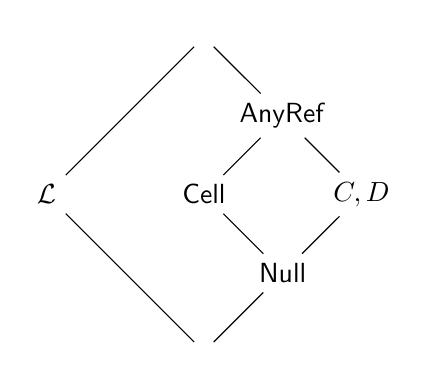
\begin{tikzpicture} 
    \node (top) at (1,3) {$\RaclTop$};
    \node (anyref) at (2,2) {\AnyRefType};
    \node (cell) at (1,1) {\CellType};
    \node (classes) at (3,1) {$C,D$};
    \node (null) at (2,0) {\NullType};
    \node (lat) at (-1, 1) {\LatType};
    \node (bot) at (1, -1) {$\RaclBot$};
    \draw (top) -- (lat) -- (bot) -- (null) -- (classes) -- (anyref) -- (top);
    \draw (anyref) -- (cell) -- (null);
  \end{tikzpicture}
  \caption{Type lattice of RACL}
  \label{fig:racl_typelat}
\end{figure}

\subsection{Terms \& Expressions}%
\label{sub:terms_and_expressions}

The basic building blocks of our type system are the typing of expressions and
terms. Our typing relation is written
\begin{equation}
  \TypeRel{\Gamma}{a}{t}{\tau} \quad \text{ or } \quad
  \TypeRel{\Gamma}{a}{e}{\tau}. \notag
\end{equation}
Apart from the usual components, i.e., typing environment $\Gamma$, term $t$ or
expression $e$ and type $\tau$, we note that it includes a designator $a$ which
can take on the values \nocap{} and \ocap{}. The latter indicates that the term
or expression is typed under OCAP constraints. This is equivalent to the OCAP
typing of \LaCasa{}~\parencite{conf/oopsla/HallerL16}. 

All typing rules for terms and expressions can be found in
Figure~\ref{fig:expr_typing}. Most of the type system rules are standard. For
example, rule {\sc T-Let} types a let-term if the subexpression $e$ is typeable
as $\tau$ under $\Gamma; a$, and the subterm $t$ is typeable under the extended
environment $\Gamma, x: \tau$ and $a$. Rule {\sc T-Var} types a variable under
$\Gamma$ provided $x \in \dom(\Gamma)$. {\sc T-New} types $\New{C}$ under effect
$a = \ocap$ only if the class $C$ is typeable as $\ocap$. The rules for typing a
class as $\ocap$ is defined in Figure~\ref{fig:ocap_typing}. Typing rule {\sc
T-Call} states that a method call $\Call{x}{m}{y}$, is only typeable if the type
of $y$ is a subtype of the method parameter type $\sigma$. {\sc T-Put} types the
expression $\Put{x}{y}$ if $x$ is typeable as \CellType{} and $y$ is of the lattice
type \LatType.

As a final example, the rule {\sc T-When} describes typing of the dependency
creation expression. It says that in order to register a callback for lattice
value $y$ in cell $x$, first $x$ and $y$ must be typeable as $\CellType$ and
$\LatType$ respectively. Furthermore all captured variables in $\overline{cap}$
must be typeable as $\CellType$. This is to ensure that all objects shared
between threads are of cell type. This is similar to capturing constraints in
spores~\parencite{conf/ecoop/MillerHO14}. Finally, the term $t$ from callback
closure $z \Rightarrow t$ must be typeable in an environment consisting of the
captured variables and $z: \LatType$.


\begin{figure}[h!]
  \centering
  %\begin{multicols}{2}
    \scrule{T-Let}
    {\TypeRel{\Gamma}{a}{e}{\tau} \andalso \TypeRel{\Gamma,x:
    \tau}{a}{t}{\sigma}}
    {\TypeRel{\Gamma}{a}{ \Let{x}{e}{t} }{\sigma}}

    \vspace{0.5em}

    \scax{T-Null}{\TypeRel{\Gamma}{a}{\NullVal}{\NullType}}

    \vspace{0.5em}

    \scax{T-LVal}{\TypeRel{\Gamma}{a}{l}{\LatType}}
    
    \vspace{0.5em}

    \scrule{T-Var}{x \in \dom(\Gamma)}{\TypeRel{\Gamma}{a}{x}{\Gamma(x)}}

    \vspace{0.5em}

    \scrule{T-Select}
    {\TypeRel{\Gamma}{a}{x}{C} \andalso \ftype(f, C) = \tau }
    {\TypeRel{\Gamma}{a}{\FSel{x}{f}}{\tau}}
    
    \vspace{0.5em}

    \scrule{T-Assign}
    {\TypeRel{\Gamma}{a}{x}{C} \andalso \ftype(f, C) = \tau \\
    \TypeRel{\Gamma}{a}{y}{\tau'} \andalso \tau' \stof \tau }
    {\TypeRel{\Gamma}{a}{\FAss{x}{f}{y}}{\tau}}

    \vspace{0.5em}

    \scrule{T-New}
    {a = \ocap \Longrightarrow \ocap(C)}
    {\TypeRel{\Gamma}{a}{\New{C}}{C}}

    \vspace{0.5em}

    \scax{T-NewCell}{\TypeRel{\Gamma}{a}{\NewCell}{\CellType}}
    
    \vspace{0.5em}

    \scrule{T-Call}
    {\TypeRel{\Gamma}{a}{x}{C} \andalso \mtype(C,m) = \sigma \to \tau \\
    \TypeRel{\Gamma}{a}{y}{\sigma'} \andalso \sigma' \stof \sigma }
    {\TypeRel{\Gamma}{a}{\Call{x}{m}{y}}{\tau}}
    
    \vspace{0.5em}

    \scrule{T-Put}
    {\TypeRel{\Gamma}{a}{x}{\CellType} \andalso \TypeRel{\Gamma}{a}{y}{\LatType}}
    {\TypeRel{\Gamma}{a}{\Put{x}{y}}{\CellType}}
    
    \vspace{0.5em}

    \scrule{T-When}
    {\TypeRel{\Gamma}{a}{x}{\CellType} \andalso \TypeRel{\Gamma}{a}{y}{\LatType} \\
    \forall \Capt{u}{u'} \in \overline{cap}. \; \TypeRel{\Gamma}{a}{u'}{\CellType}\\
    \Gamma_{\text{cells}} = [u \mapsto \CellType : \Capt{u}{u'} \in \overline{cap}]\\
    \TypeRel{\Gamma_{\text{cells}}, z : \LatType}{\ocap}{t}{\sigma}}
    { \TypeRel{\Gamma}{a}{\When{x}{y}{ \CB{\overline{cap}}{z}{t}}}{\CellType} }

  %\end{multicols}
  \caption{\RACL{} typing rules for expressions and terms.}
  \label{fig:expr_typing}
\end{figure}

\subsection{Well Formed Programs}%
\label{sub:well_formed_programs}

Intuitively, a well formed program is a program which obeys our type system. We
define well-formedness in Figure~\ref{fig:wf_typing}. We also need the
definition of the global typing environment $\Gamma_0$. 
\begin{definition}
  Let the \emph{global typing environment} $\Gamma_0$ be defined as 
  \begin{equation*}
    \Gamma_0 = \Global : C_g
  \end{equation*}
\end{definition}
{\sc WF-Prog} says that in order for a program $p =
\overline{cd}~\overline{vd}~t$ to be well typed, all classes $\overline{cd}$,
global variables $\overline{vd}$ and the program term $t$ must be well formed.
Rule {\sc WF-Global} says that in order for a global variable declaration to be
well formed, the denoted type must either be $\LatType$, $\CellType$ or be of
class type $C$ where the class definition of $C$ is well formed. In order for a
class definition of $C$ to be well formed, rule {\sc WF-Class} declares that all
methods must be well formed under $C$, the extended class $D$ must either be
$\AnyRefType$ or must also be well formed. Furthermore, all methods must obey the
rules of overriding and $C$ cannot redeclare any fields that has been declared
in an extended class $D$. {\sc WF-Override} declares that for a method to be
correctly overriden it must either not be declared in any extended class or it
must have the same declared type as in the extended class. Finally {\sc
WF-Method} states that in order for a method to be well formed, its term must be
typable as a type $\tau'$ under an environment consisting of the global
environment, the class itself $\This : C$ and the method parameter $x: \sigma$.
Futhermore $\tau' \stof \tau$, where $\tau$ is the declared return type of the
method.



\begin{figure}[h]
  \scrule{WF-Prog}
  {p \vdash \overline{cd} \andalso p \vdash \overline{vd} \andalso
  \TypeRel{\Gamma_0}{\nocap}{t}{\tau}}
  {p \vdash \overline{cd} \: \overline{vd} \: t}

  \RuleSpace{}

  \scrule{WF-Global}
  {\sigma = \LatType \lor \sigma = \CellType ~ \lor  \\
  (\sigma = C \land p \vdash \ClassDef{C}{...}{...}{...})}
  {p \vdash \VarDecl{f}{\sigma}}
  
  \RuleSpace{}

  \scrule{WF-Class}
  {C \vdash \overline{md} \\ D = \AnyRefType{} \lor
  p \vdash \ClassDef{D}{...}{...}{...} \\
  \forall (\MethodDef{m}{...}{...}{...}{...}) \in \overline{md} . \: \override(m,
  C, D) \\
  \forall (\VarDecl{f}{\tau}) \in \overline{vd} . \: f \notin \fields(D) }
  {p \vdash \ClassDef{C}{D}{\overline{vd}}{\overline{md}}}

  \RuleSpace{}

  \scrule{WF-Override}
  {\mtype(m, D)\text{ not def. } \lor \mtype(m, C) = \mtype(m, D)}
  {\override(m, C, D)}
  
  \RuleSpace{}

  \scrule{WF-Method}
  { \TypeRel{\Gamma_0, \This:C, x : \sigma}{\nocap}{t}{\tau'} \\
  \tau' \stof \tau}
  {C \vdash \MethodDef{m}{x}{\sigma}{\tau}{t}}
  \caption{\RACL{} rules for well formedness of programs.}
  \label{fig:wf_typing}
\end{figure}

\subsection{OCAP Typing}%
\label{sub:ocap_typing}

In Figure~\ref{fig:ocap_typing} we find the rules for classifying a type as $\ocap$.
Immediately we see that unconditionally, both $\AnyRefType$ and $\CellType$ are
$\ocap$. To type a class $C$ as $\ocap$, {\sc OCAP-Class} says that apart from being
well formed, the superclass $D$ must be $\ocap$. Furthermore, all methods must
be typable under the special judgement $\vdash_{\ocap}$ and all fields must be
$\ocap$.  For a method to be typed under $\vdash_{\ocap}$, rule {\sc
OCAP-Method} declares that the method term must be typable under effect $\ocap$
without access to the global environment $\Gamma_0$. Being typable under effect
$\ocap$ means that expression $\New{C}$ is only allowed if $C$ is $\ocap$, as
stated in rule {\sc T-New}. In short, an ocap term can only instansiate ocap
classes. This part of the type system is similar to the corresponding part of
LaCasa~\parencite{conf/oopsla/HallerL16}.

\begin{figure}
  \scax{OCAP-AnyRef}
  {\ocap{(\AnyRefType{})}}

  \RuleSpace{}

  \scax{OCAP-Cell}
  {\ocap(\CellType)}

  \RuleSpace{}

  \scrule{OCAP-Class}
  {\ocap{(D)} \andalso C \vdash_{\ocap} \overline{md} \\
  \forall (\VarDecl{f}{\sigma}) \in \overline{vd}. \: ocap(\sigma)}
  {\ocap{(C)}}

  \RuleSpace{}

  \scrule{OCAP-Method}
  {\TypeRel{\This : C, x : \sigma}{\ocap}{t}{\tau'} \\
  \tau' \stof \tau}
  {C \vdash_{\ocap} \MethodDef{m}{x}{\sigma}{\tau}{t}}
  \caption{\RACL{} OCAP rules.}
  \label{fig:ocap_typing}
\end{figure}


\section{Properties}
\label{sec:properties}

In order to state and prove things such as progress and preservation we need a few more
definitions. Many of them are just auxilliary properties of things like states
and types and build up to the final definition of a well typed state.

\subsection{Well Typed Heap}%
\label{sub:well_typed_heap}

This first definition is a straightforward partial function defining the dynamic
type of a value.
\begin{definition}
  The partial function $\typeOf$ is defined as follows:
  \begin{equation}
    \typeOf{(k, H)} =
    \begin{cases}
      \LatType, &\text{ if }k \in \LatVals \\
      \NullType, &\text{ if }k = \NullVal \\
      \CellType, &\text{ if }k \in \dom{(H)}\text{ and } H(k) = \Cell{...} \\
      C, &\text{ if }k \in \dom{(H)}\text{ and } H(k) = \Obj{C, ...} \\
    \end{cases}
  \end{equation}
\end{definition}
In order to simplify the definition of a well typed heap we define the
following.
\begin{definition}
  The typing environment $\Gamma_{\CellType}(L)$ is defined as follows:
  \begin{equation}
    \Gamma_{\CellType}(L) = \left[(x: \CellType) : x \in \dom(L)\right]
  \end{equation}
\end{definition}
Next comes the definition of a well typed heap. To say that a heap is
well typed intuitively means that for all class objects, all field values are of
a subtype of the declared type. Furthermore, our definition includes a statement
about cell objects. We say that for all callbacks stored in dependency sets, all
captured values must be of cell type and the callback term must be typeable
under an environment containing the captured variables and closure parameter
$z$.
\begin{definition}[Well Typed Heap]
  A heap $H$ is well typed, written $\vdash{H}$, if
  $\forall o \in \dom{(H)}$:

  If $H(o) = \Obj{C, FM}$ then
  \begin{equation} \label{eq:defwth1}
    \begin{aligned}
      \forall f &\in \fields{(C)}. \\ 
      &f \in \dom{(FM)} \: \land \\ 
      &\typeOf{(FM(f), H)} \stof \ftype{(f, C)}
    \end{aligned}
  \end{equation}
  and if $H(o) = \Cell{DEP, l}$ then
  \begin{equation} \label{eq:defwth2}
    \begin{aligned}
      \forall (l'&, (L_{\text{env}}, z \Rightarrow t))^\iota \in DEP. \\
      &\forall (x \mapsto k) \in L_{\text{env}}.\: \typeOf{(k, H)} \stof
      \CellType \: \land \\
      &\TypeRel{\Gamma_{\CellType{}}(L_{\text{env}}), z:
      \LatType}{\ocap}{t}{\gamma} 
    \end{aligned}
  \end{equation}
\end{definition}

\subsection{Well Typed Threads}%
\label{sub:well_typed_threads}

A non erroneous state $S = H, P$ has two parts. In order to define and
prove preservation properties, we furthermore need to put restrictions on the
thread set $P$. We do this with the relation $H \vdash P$, saying $P$ is well
typed under heap $H$. This relation is defined in Figure~\ref{fig:ts_typing}.
{\sc T-Procs} and {\sc T-Empty} basically says that in order for a thread set
$P$ to be well typed under heap $H$, all threads needs to be well typed under
$H$ and its OCAP status $a$.  For a thread $GS|_a^\iota$ we write this as $H; a
\vdash GS$. This relation is defined in Figure~\ref{fig:fs_typing}. 

For $H; a \vdash GS$ to hold, either $FS = \varepsilon$ as in rule {\sc
T-FSEmpty1} (this is actually impossible since frame stacks of a state cannot be
empty, see definition~\ref{def:thread_sets}), or the term $t$ of top frame $F$
is typeable with some environment $\Gamma$ which is conformant with its local
variable map $L$ and $H$. This conformancy is expressed through the relation $H
\vdash \Gamma; L$ which is defined in Figure~\ref{fig:local_typing}. Simply
stated, it says that all types specified in $\Gamma$ aligns with the dynamic
types of the values in $L$. Furthermore {\sc T-FS1} declares that the rest of the frame
stack $FS$ must be typable under the judgement $\vdash^{x: \sigma}$. This
judgement is defined by rules {\sc T-FSEmpty2} and {\sc T-FS2}. The latter
reflects that the top frame returns some value to its underlying frame stack. It
is closely connected with the well-formedness of methods and call\slash return
execution semantics as defined by rules {\sc WF-Method} and \ECall{}\slash\ERet{}
respectively.

\subsection{Isolation}%
\label{sub:isolation}

The next two definitions are used when defining isolation of threads in the
reference graph of the heap. The ruling accRoot(o, FS) is defined in
Figure~\ref{fig:def_accroot}.
\begin{definition}[Class Object Separation]
  For any heap $H$ and heap references $o, o'$ we have class object separation,
  $\csep{(H, o, o')}$ iff
  \begin{align}
    \label{eq:csep_def}
    \forall q, q' &\in \dom{(H)}. \notag\\
    & \reach{(H, o, q)} \: \land \: \reach{(H, o', q')} \implies \notag\\ 
    &q \neq q' \: \lor \typeOf{(q, H)} = \CellType
  \end{align}
\end{definition}

\begin{definition}[Accessible Roots]
  For a heap $H$ and a frame stack $FS$ we define $\accRoots{(FS, H)}$ as
  \begin{equation}
    \accRoots{(FS, H)} = \left\{ o \in \dom{(H)}: \accRoot{(o, FS)} \right\}
  \end{equation}
\end{definition}

Isolation of threads is defined in Figure~\ref{fig:def_isolation}. Rule {\sc
ISO-FS} states that for two threads to be isolated with regards to heap $H$, all
accessible roots of the two threads must have class object separation, i.e. that
all objects that are reachable from both threads must be of type $\CellType$.
Rule {\sc ISO-Procs} states that we have isolation for a thread set $P$ under
heap $H$, if there is isolation between all pair of threads such that at least
one is $\ocap$.

\subsection{OCAP Reachability}%
\label{sub:ocap_reachability}

In order to prove preservation of isolation we also need to ensure that all
objects reachable from an $\ocap$-annotated thread can be typed as an $\ocap$
type. The next definition together with Figure~\ref{fig:def_ocapreach} defines
this property formally.
\begin{definition}[OCAP Reachability]
  For a heap $H$ and frame stack $FS$ we have $\ocrloc{(FS,H)}$ iff
  \begin{align}
    \label{eq:ocr_def}
    \forall o \in \: &\accRoots(FS,H), o' \in \dom(H). \notag\\
    &\reach{(H, o, o')} \implies \ocap{(\typeOf{(o', H)})}
  \end{align}
\end{definition}

\subsection{Global Object Separation}%
\label{sub:global_object_separation}

Another thing needed to prove preservation of isolation is global object
separation. Simply stated this means that no $\ocap$ thread can reach the global
object $o_g$ through heap references. This is formally defined in
Figure~\ref{fig:def_gsep}.

\subsection{No Thread Spawning}%
\label{sub:no_thread_spawning}

The next definition is needed to state and prove progress.
\begin{definition}[No Spawn]
  For any heap $H$ we have $\noSpawn(H)$ if and only if
  \begin{equation}
    \begin{aligned}
      \forall o &\in \dom(H). \\
        & H(o) = \Cell{DEP, l} \implies 
        \forall (l', cb)^\iota \in DEP. \: \lnot (l' \sqsubseteq l).
    \end{aligned}
  \end{equation}
\end{definition}

\subsection{Unique Main Thread}%
\label{sub:unique_main_thread}

In order to prove determinism we must be sure that there is at most one
non-$\ocap$ thread running. Otherwise these could interfere since there are no
constraints on whether these can share data. Therefore we define the following
property.
\begin{definition}[Unique Main Thread]
  For a thread $FS|_a^\iota$ let
  \begin{equation*}
    \chi_{\nocap}(a) =
    \begin{cases}
      1 & \text{ if } a = \nocap \\
      0 & \text{ o.w. }
    \end{cases}
  \end{equation*}
  For a thread set $P$ let
  \begin{equation*}
    \chi(P) = \sum_{FS|_a^\iota \in P} \chi_{\nocap}(a).
  \end{equation*}
  This is the number of non OCAP protected threads in $P$. Finally we define
  \begin{equation*}
    \uniqMain(P) \iff \chi(P) \leq 1
  \end{equation*}
\end{definition}


\subsection{Well Typed States}%
\label{sub:well_typed_states}

Finally we can define the notion of a well typed state. This combines many of
the properties already defined into one.
\begin{definition}[Well Typed States]
  For a state $S$ we say that it is well typed, written
  \begin{equation}
    \vdash S \tsep \stateok
  \end{equation}
  if $S = \Error$ or $S = H, P$ and
  \begin{equation*}
    \begin{gathered}
      \vdash H \andalso H \vdash P \andalso H \vdash P \tsep \ocr \\
      \isolation{(H, P)} \andalso H \vdash P \tsep \gsep \andalso \uniqMain(P)
    \end{gathered}
  \end{equation*}
  
\end{definition}

\begin{figure}
  \scrule{WF-EnvVar}
  {\typeOf{(L(x), H) \stof \Gamma{(x)}}}
  { H \vdash \Gamma; L; x }

  \RuleSpace{}

  \scrule{WF-Env}
  {\dom{(\Gamma)} \subseteq \dom{(L)} \\
    \forall x \in \dom{(\Gamma)}. \: H \vdash \Gamma; L; x 
  }
  { H \vdash \Gamma; L }

  \caption{Rules for classifying local environments $L$ as well typed.}
  \label{fig:local_typing}
\end{figure}

\begin{figure}
  \scax{T-FSEmpty1}
  {H; a \vdash \varepsilon}

  \RuleSpace{}

  \scax{T-FSEmpty2}
  {H; a \vdash^{x : \sigma} \varepsilon}

  \RuleSpace{}

  \scrule{T-FS1}
  { F = \Frame{L}{t}{x} \andalso H \vdash \Gamma; L \\
  \TypeRel{\Gamma}{a}{t}{\sigma'} \andalso \sigma' \stof \sigma \andalso H; a \vdash^{x: \sigma} FS }
  { H; a \vdash F \circ FS }
  
  \RuleSpace{}

  \scrule{T-FS2}
  { F = \Frame{L}{t}{y} \andalso H \vdash \Gamma; L \\
  \TypeRel{\Gamma, x: \tau}{a}{t}{\sigma'} \andalso \sigma' \stof \sigma 
  \andalso H; a \vdash^{y: \sigma} FS }
  { H; a \vdash^{x: \tau} F \circ FS }

  \caption{Rules for typing frame stacks under some heap $H$ and effect $a$.}
  \label{fig:fs_typing}
\end{figure}

\begin{figure}
  \scax{T-Empty}
  {H \vdash \emptyset}

  \RuleSpace{}

  \scrule{T-Procs}
  { H; a \vdash FS \andalso H \vdash P }
  { H \vdash P \cup \left\{FS |_a^\iota \right\} }

  \caption{Rules for typing thread sets and the special value \Error{} under some heap $H$.}
  \label{fig:ts_typing}
\end{figure}

\begin{figure}
  \scrule{ISO-FS}
  { 
    \forall o \in \accRoots(FS), o' \in \accRoots(GS) . \: \csep{(H, o, o')}
  }
  {
    \isolated{(H, FS, GS)}
  }
  
  \RuleSpace{}

  \scrule{ISO-Procs}
  {
    \forall FS|_a^\iota, GS_b^{\iota'} \in P \text{ where } FS|_a^\iota \neq
    GS|_b^{\iota'} . \\
    a = \ocap \: \lor \: b = \ocap \implies \isolated{(H, FS, GS)}
  }
  {
    \isolation{(H, P)}
  }
  \caption{Definition of isolation}
  \label{fig:def_isolation}
\end{figure}

\begin{figure}
  \scrule{Reach1}
  {o \in \dom{(H)}}
  {\reach{(H, o, o)}}

  \RuleSpace{}

  \scrule{Reach2}
  {
    o \in \dom{(H)} \andalso H(o) = \Obj{C, FM} \\
    o'' \in \image{(FM)} \andalso \reach{(H, o'', o')}
  }
  { \reach{(H, o, o')} }
  \caption{Definition of reach}
  \label{fig:def_reach}
\end{figure}

\begin{figure}
  \scrule{AR-F}
  { (x \mapsto o) \in L }
  { \accRoot{(o, \sFrame{L}{t})} }

  \RuleSpace{}

  \scrule{AR-FS}
  { \accRoot{(o, F)} \: \lor \: \accRoot{(o, FS)} }
  { \accRoot{(o, F \circ FS)} }
  \caption{Definition of accRoot}
  \label{fig:def_accroot}
\end{figure}

\begin{figure}
  \scrule{OCR-FS}
  { a = \ocap \implies \ocrloc(FS, H) }
  { H; a \vdash FS \tsep \ocr }

  \RuleSpace{}

  \scax{OCR-PEmpty}
  {H \vdash \emptyset \tsep \ocr}

  \RuleSpace{}

  \scrule{OCR-P}
  {H \vdash P \tsep \ocr \andalso H; a \vdash FS \tsep \ocr}
  {H \vdash P \cup \left\{ FS|_a^\iota \right\} \tsep \ocr}

  \caption{Definition of OCAP reachability}
  \label{fig:def_ocapreach}
\end{figure}

\begin{figure}
  \scrule{GSep-Threads}
  {\forall FS|_a^\iota \in P. \: a = \ocap \implies \forall o \in \accRoots{(FS, H)}. \: \csep{(H, o, o_g)} }
  {H \vdash P \tsep \gsep}

  \caption{Definition of global separation}
  \label{fig:def_gsep}
\end{figure}

% TODO include the \Gamma_{\CellType} definition somewhere


% Introduce the core language with syntax, type system and state properties like
% WT heap, isolation, well typed state




\chapter{Preservation and Progress}
\label{cha:preservation_and_progress}

% Write about the basic ideas behind the proof of preservation and progress

\chapter{Proof of Determinism}
\label{cha:proof_of_determinism}

% Describe:
% Theorem of determinism
% Lemmas leading up to the proof of this

\chapter{Discussion \& Conclusion}
\label{cha:disc_concl}

% Discuss the addition of quiescence in order to actually use the result of the
% computation. Also discuss the efficiency of our system. In order to make it
% usable we need to replace the threshold checks with some callback that spawns
% the required callbacks. This of course is also required to not depend on any
% shared mutable state.
% Discuss threshold reads: Could introduce a get stmt. Draw some
% conclusions of the problematic nature of deterministic concurrency and that
% great care has to be taken when trying to prove determinism for so called
% "deterministic-by-design" systems.
% SHould also

\printbibliography[heading=bibintoc] % Print the bibliography (and make it appear in the table of contents)

\appendix

\chapter{Full Proofs}

\end{document}
